\documentclass[11pt,]{article}
\usepackage[left=1in,top=1in,right=1in,bottom=1in]{geometry}
\newcommand*{\authorfont}{\fontfamily{phv}\selectfont}
  \usepackage[]{mathpazo}
  
  
  \usepackage[T1]{fontenc}
\usepackage[utf8]{inputenc}




\usepackage{abstract}
\renewcommand{\abstractname}{}    % clear the title
\renewcommand{\absnamepos}{empty} % originally center

\renewenvironment{abstract}
{{%
  \setlength{\leftmargin}{0mm}
  \setlength{\rightmargin}{\leftmargin}%
}%
  \relax}
{\endlist}

\makeatletter
\def\@maketitle{%
  \newpage
  %  \null
  %  \vskip 2em%
    %  \begin{center}%
    \let \footnote \thanks
  {\fontsize{18}{20}\selectfont\raggedright  \setlength{\parindent}{0pt} \@title \par}%
}
%\fi
\makeatother


  
  
  \setcounter{secnumdepth}{0}

          
    \usepackage{graphicx,grffile}
\makeatletter
\def\maxwidth{\ifdim\Gin@nat@width>\linewidth\linewidth\else\Gin@nat@width\fi}
\def\maxheight{\ifdim\Gin@nat@height>\textheight\textheight\else\Gin@nat@height\fi}
\makeatother
% Scale images if necessary, so that they will not overflow the page
% margins by default, and it is still possible to overwrite the defaults
% using explicit options in \includegraphics[width, height, ...]{}
\setkeys{Gin}{width=\maxwidth,height=\maxheight,keepaspectratio}
  
  
    \title{Incorporating spatial components into reflectance-based models of
suspended solids improves predictive performance  }
  
  
  
  \author{\Large Sean Hardison\vspace{0.05in} \newline\normalsize\emph{University of Virginia}  }
  
  
  \date{}

\usepackage{titlesec}

\titleformat*{\section}{\normalsize\bfseries}
\titleformat*{\subsection}{\normalsize\itshape}
\titleformat*{\subsubsection}{\normalsize\itshape}
\titleformat*{\paragraph}{\normalsize\itshape}
\titleformat*{\subparagraph}{\normalsize\itshape}


  
      
  
  \newtheorem{hypothesis}{Hypothesis}
\usepackage{setspace}


% set default figure placement to htbp
\makeatletter
\def\fps@figure{htbp}
\makeatother

  \usepackage{float} \usepackage{longtable} \usepackage{caption} \usepackage{setspace}\doublespacing
    
  % move the hyperref stuff down here, after header-includes, to allow for - \usepackage{hyperref}

\makeatletter
\@ifpackageloaded{hyperref}{}{%
  \ifxetex
  \PassOptionsToPackage{hyphens}{url}\usepackage[setpagesize=false, % page size defined by xetex
                                                 unicode=false, % unicode breaks when used with xetex
                                                 xetex]{hyperref}
  \else
    \PassOptionsToPackage{hyphens}{url}\usepackage[draft,unicode=true]{hyperref}
  \fi
}

\@ifpackageloaded{color}{
  \PassOptionsToPackage{usenames,dvipsnames}{color}
}{%
  \usepackage[usenames,dvipsnames]{color}
}
\makeatother
\hypersetup{breaklinks=true,
bookmarks=true,
pdfauthor={Sean Hardison (University of Virginia)},
pdfkeywords = {},  
pdftitle={Incorporating spatial components into reflectance-based models of
suspended solids improves predictive performance},
colorlinks=true,
citecolor=blue,
urlcolor=blue,
linkcolor=magenta,
pdfborder={0 0 0}}
\urlstyle{same}  % don't use monospace font for urls

% Add an option for endnotes. -----


% add tightlist ----------
\providecommand{\tightlist}{%
\setlength{\itemsep}{0pt}\setlength{\parskip}{0pt}}

% add some other packages ----------

% \usepackage{multicol}
% This should regulate where figures float
% See: https://tex.stackexchange.com/questions/2275/keeping-tables-figures-close-to-where-they-are-mentioned
\usepackage[section]{placeins}


\begin{document}
	
% \pagenumbering{arabic}% resets `page` counter to 1 
%
% \maketitle

{% \usefont{T1}{pnc}{m}{n}
\setlength{\parindent}{0pt}
\thispagestyle{plain}
{\fontsize{18}{20}\selectfont\raggedright 
\maketitle  % title \par  

}

{
   \vskip 13.5pt\relax \normalsize\fontsize{11}{12} 
\textbf{\authorfont Sean Hardison} \hskip 15pt \emph{\small University of Virginia}   

}

}








\begin{abstract}

    \hbox{\vrule height .2pt width 39.14pc}

    \vskip 8.5pt % \small 

\noindent Reflectance-based models of water quality are popular due to the high
temporal and spatial coverage provided by satellite imagery. However,
such models are limited by the availability of \emph{in situ} match-up
data that can be used to groundtruth models. In cases when match-ups are
sparse, regression models may be biased by the presence of spatially
autocorrelated residuals, potentially leading to misleading predictions.
Here we compare the predictive performance of four different
reflectance-based regression models of total suspended solids (TSS) in
Chesapeake Bay. Results showed that models incorporating spatial
components performed better in prediction tasks than those that did not.
We next applied the best fitting models to a similar but
hydrodynamically unique ecosystem to explore model transferrability, but
found that the models were not effective in predicting TSS in the new
ecosystem; likely due to biases in the model training procedure.
Regardless, we found that incorporating spatial components into
reflectance-based models of TSS can improve their predictive capacity
and therefore their utility to resource managers.


    \hbox{\vrule height .2pt width 39.14pc}


\end{abstract}


\vskip -8.5pt


 % removetitleabstract

\noindent  

\linespread{1.25}

\hypertarget{introduction}{%
\section{Introduction}\label{introduction}}

The use of regression models to relate remotely sensed surface
reflectance to water quality parameters is a popular method of
environmental monitoring worldwide (Park and Latrubesse 2014; Ouma,
Noor, and Herbert 2020; Matus-Hernandez, Hernández-Saavedra, and
Martínez-Rincón 2018). These models are often derived opportunistically
from match-ups between water quality sampling and satellite fly-overs
(e.g.~Luis et al. 2019), which may be limiting in areas where water
quality measurements are difficult to frequently ascertain. In such
cases, water quality observations may be clustered in space or time, and
the use of such measurements in reflectance-based regression models may
introduce autocorrelated errors. While such a model may have high
explanatory power, its ability to predict over new data, and therefore
its utility to resource managers, will likely be hampered due to the
presence of biased estimates.

The presence of spatial autocorrelation in environmental data is so
common that is has been enshrined in Tobler's First Law of Geography:
``everything is related to everything else, but near things are more
related than distant things'' (Tobler 1970; Miller 2004). It follows
that metrics of water quality are also autocorrelated; for example, the
concentration of total suspended solids (TSS) in the water column will
be more similar to TSS concentration at a site nearby than at a site
further away. This is most clearly evidenced by the formation of
sediment plumes flowing into estuaries after large storm events, such as
the large plume that traveled southwards into Chesapeake Bay from the
Susquehanna River following Tropical Storm Lee in 2011 (Hirsch 2012).
The plume created a spatial dependence structure in suspended sediment
concentrations along a North-South gradient as it flowed into the Bay:
sediment concentrations would have been highly correlated with one
another in the center of the plume and the correlation would have
degraded with distance outwards.

On a less extreme scale, there are several physical mechanisms to
consider that contribute to TSS loading in Chesapeake Bay and its
surrounding estuaries. TSS concentrations are generally highest within
the tributaries of Chesapeake Bay (Son and Wang 2012). Sediments can be
mobilized by rain events or development upstream in a surrounding
tributary, subsequently leading to deposition of the larger sediment
size fractions near river mouths. Smaller diameter sediment fractions
will flow into the mainstem of the Bay, but in lower concentrations. In
nearby coastal estuaries, such as the coastal bays of Virginia, the
hydrodynamic environment is more influenced by waves, tides, and
vegetation than by riverine inflow (Nardin, Lera, and Nienhuis 2020).
These environmental drivers contribute to spatial autocorrelation of
suspended sediments, and more broadly TSS, on small to regional scales
that could potentially lead to biased predictions if reflectance-based
regression models are developed using sparse validation data.

In this paper, we compare the predictive performance of four
reflectance-based regression models of TSS in Chesapeake Bay. We
hypothesized that the inclusion of spatial information in regression
models would improve predictions on out-of-sample test data. We also
tested the transferrability of the best fitting models by applying them
to TSS data collected in the Virginia Coast Reserve along the Atlantic
coast of Virginia.

\hypertarget{methods}{%
\section{Methods}\label{methods}}

\hypertarget{total-suspended-solids-data}{%
\subsection{Total suspended solids
data}\label{total-suspended-solids-data}}

Total suspended solids (TSS) data were queried from water quality
databases hosted by the Chesapeake Bay Program
(\url{https://www.chesapeakebay.net/what/publications_and_data}) and the
Virginia Coast Reserve Long-term Ecological Research program (VCR LTER;
\url{https://www.vcrlter.virginia.edu/cgi-bin/showDataset.cgi?docid=knb-lter-vcr.247}).
In both cases, water samples of pre-determined volume were filtered
through paper filters, dried, and then weighed to estimate the dry
weight of suspended solids in the sample. Only TSS samples collected in
the upper 2 m of the water column were considered in this analysis. TSS
data were collected from 59 monitoring stations in Chesapeake Bay, and
from six stations in the Virginia Coast Reserve (VCR) (Fig. 1). In
Chesapeake Bay, the queried data were limited to samples occurring on
the same day as a MODIS-Terra fly-over between 2000-02-24 and
2020-07-30. However, there were only 16 same-day water quality-MODIS
match-ups over the study period in the VCR, so we counted a match-up as
a MODIS flyover within one day of water quality sampling. This increased
our sample size to 48 match-ups in the VCR.

\begin{figure}
\centering
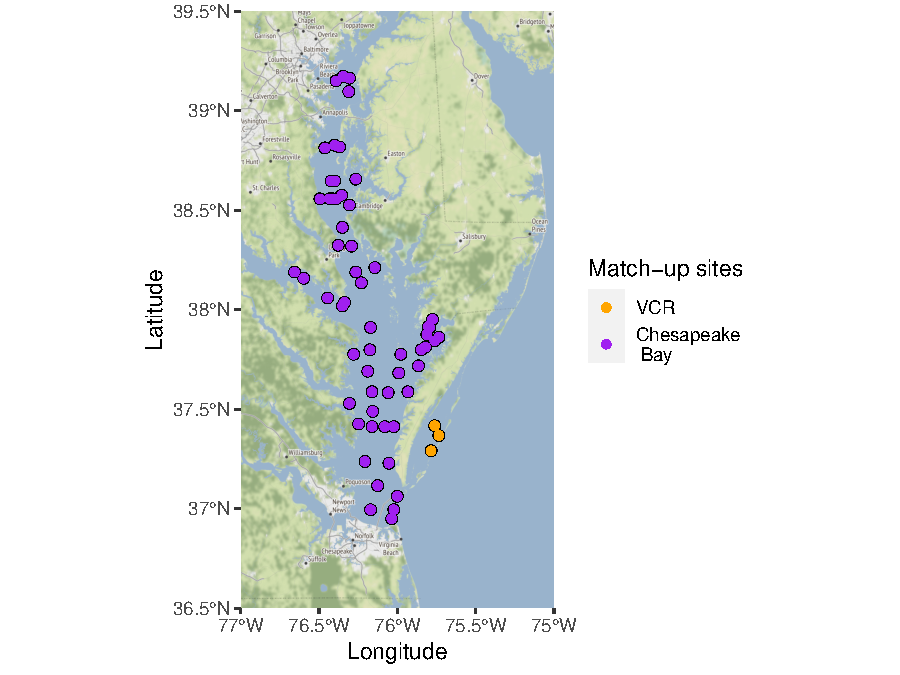
\includegraphics{ssrs_sp2020_files/figure-latex/cb-map1-1.pdf}
\caption{Locations of water quality-MODIS Terra match-up sites in
Chesapeake Bay (purple) and in the Virginia Coast Reserve (orange).}
\end{figure}

\hypertarget{modis-terra-reflectance-data}{%
\subsection{MODIS-Terra reflectance
data}\label{modis-terra-reflectance-data}}

Match-ups between the L3 Ocean Color SMI (L3SMI) 500 m resolution
MODIS-Terra product and water quality sampling events over the period of
2000-02-24 - 2020-07-30 were identified using Google Earth Engine. The
L3SMI product is available for public use with a previously applied land
mask, scale factor, and offsets. We used surface reflectance from the
645 nm band for regression analyses, as this band has been successfully
used for similar applications in riverine environments (Park and
Latrubesse 2014). We identified 451 unique images that included one or
more pixel match-up with water quality sampling events in Chesapeake
Bay, yielding 1761 matches in total. In the VCR, we identified 27 unique
images that matched water quality sampling events within a day, yielding
48 observations in total.

\hypertarget{model-building}{%
\subsection{Model building}\label{model-building}}

We developed four models of varying complexity to predict TSS from
reflectance data. The first model was a linear regression model of the
form

\[TSS_{i} = \alpha + \beta_{1}\times Rrs_i + \epsilon_{i},\] where
\(TSS_i\) is a unique TSS indexed by the combination of date and site
(\(i\)), \(\alpha\) is the model intercept, \(\beta_{1}\) is the slope,
\(Rrs_{i}\) is the remote sensing reflectance, and \(\epsilon_{i}\) is
an error term assumed to be normally distributed with mean 0 and
variance \(\sigma^2\).

The second model was a generalized linear model (GLM) with a log-link
assuming \(TSS_i\) to be gamma distributed, but was otherwise identical
in covariates to the simpler regression model. We chose to model \(TSS\)
as gamma distributed because the gamma GLM minimized deviations from
expected residual patterns in model diagnostics. The GLM was given by
\[\log ({ E(TSS_{i}) })  = \alpha + \beta_{1}\times Rrs_i.\] The gamma
distribution was appropriate in this case because it is specifically
used to model continuous data that are greater than 0. Given the
expected value \(E(TSS_i) = \mu\), the distribution variance is
\(\frac{\mu^2}{v}\), where \(v\) is a dispersion parameter (Zuur et al.
2009). We fitted GLMs in R using the \emph{MASS} package (Venables and
Ripley 2002).

The third model we tested was a generalized additive model (GAM) with an
identity link, which allowed for non-linearity in the model of \(TSS\).
We also included a second covariate in this model to explicitly account
for spatial variability along latitudinal and longitudinal environmental
gradients in Chesapeake Bay TSS; represented by the interaction of water
quality sampling site latitude and longitude. The model was

\[E(TSS_{i}) = \beta_0 + f_1(Rrs_{i}) + f_{2}(lon_{i}, lat_{i}),\] where
\(f_{1}\) is a smooth function of remote sensing reflectance, and
\(f_{2}\) is the tensor product of longitude and latitude at site and
day \(i\) (Pedersen et al. 2019). GAMs were fitted using the R package
\emph{mgcv} (Wood 2011).

The final model was a spatial generalized linear mixed effects model
(GLMM) with an identity link. Similarly to the GAM, this model
explicitly accounted for the effect of space on TSS, but did so by
modeling space as a random effect using Gaussian random fields (GRFs).
This type of model, which is also known as a predictive process model,
has been shown to have a predictive edge when compared to regression
models with spatial trend components (e.g.~the GAM described above)
(Latimer et al. 2009). By explicitly modeling spatial autocorrelation,
predictive process models can also generate reasonable predictions over
unmeasured space using methods similar to kriging.

The model is a two-stage hierarchical model, where the first stage
relates \(TSS\) to \(Rrs\) and a spatial component representing a vector
of spatially correlated errors, \(W\). Modeling \(W\) at each location
\(n\) is computationally expensive, and so the second stage of the model
involves specifying a spatial process across a reduced domain given by
\(m\) knots (Fig. 2). The spatial process estimated at \(m\) knots,
\(W*\), is given by a multivariate normal distribution

\[W^* \sim MVN(0, \Sigma^*),\] where \(\Sigma^*\) is a covariance matrix
describing the isotropic spatial association between knots (i.e.~the
association varies only with distance, not direction). The spatial
random effects at each water quality sampling location (\(W\)) can then
be estimated from the reduced representation \(W^*\) using a method
similar to kriging (Latimer et al. 2009; Anderson and Ward 2019). The
full model is given by

\[E(TSS_{i}) = \beta_0 + \beta_{1}\times Rrs_{i} + w_{i},\] where
\(w_{i}\) is an element in the vector \(W\) describing a spatial random
effect for site and date \(i\). We fitted spatial GLMMs using the
\emph{sdmTMB} and \emph{INLA} R packages (Rue, Martino, and Chopin 2009;
Anderson et al. 2020; R Core Team 2020). All code used in this analysis
is available at \url{https://github.com/seanhardison1/ssrs}.

\begin{figure}

{\centering \includegraphics[trim={0 2.25cm 0 2.25cm},clip]{ssrs_sp2020_files/figure-latex/inla-mesh-1} 

}

\caption{The reduced spatial domain over which the spatial process $W^*$ is modeled. Each intersection of the mesh within the blue polygon represents a knot.}\label{fig:inla-mesh}
\end{figure}

\hypertarget{model-evaluation}{%
\subsection{Model evaluation}\label{model-evaluation}}

Model performances were evaluated by cross validation, in which the the
full TSS-Rrs data set was randomly subsetted into training and testing
sets containing 80\% and 20\% of the original data respectively. Each
model was fitted using the training set and then applied to the test
set. Prediction performance on the test set was measured using root mean
square error (RMSE). This procedure was performed 10 times on 10 unique
data subsets to explore the performance of each model. The best two
models, which minimized RMSE across the cross validation exercises, were
then applied to the VCR TSS-Rrs data set to evaluate model
transferrability.

\hypertarget{results}{%
\section{Results}\label{results}}

Our analysis revealed that accounting for spatial processes in
reflectance-based models of TSS improves the performance of
out-of-sample prediction (Fig. 3). There was an \textasciitilde5.8\%
decrease in prediction error between the best-performing GAM and worst
performing GLM model, whereas the difference in mean RMSE between the
GAM and spatial GLMM was only \textasciitilde0.3\%. The simple linear
model performed better than the gamma distributed GLM, with a
\textasciitilde3.9\% decrease in prediction error between the two
models. While out-of-sample performance was high across models, the best
performing models performed poorly when transferred to the VCR ecosystem
(Fig. 4). Model predictions in the VCR largely underestimated TSS from
water quality sampling.

\begin{figure}
\centering
\includegraphics{ssrs_sp2020_files/figure-latex/cross-val-1.pdf}
\caption{Results from cross-validation of reflectance-based models of
TSS showing mean prediction error in terms of RMSE by model. Bars show
bootstrapped 95\% confidence intervals for the sample mean.}
\end{figure}

\begin{figure}
\centering
\includegraphics{ssrs_sp2020_files/figure-latex/oot-perf-1.pdf}
\caption{Model prediction performance on an out-of-system test set in
the VCR (top row) and an out-of-sample test set in the Chesapeake Bay
(bottom row). The orange lines are linear regressions to show deviation
from the 1:1 line, shown in black.}
\end{figure}

To further compare outputs from the spatial GLMM and GAM, we used the
two models to predict TSS over the Chesapeake Bay spatial domain from a
single MODIS image on June 5th, 2010 (Fig. 5). Comparing the two
predictions illustrates how the models treat their respective spatial
components. Qualitatively, the GAM appears to put more weight on the
longitudinal gradient in TSS than the spatial GLMM, and predicts higher
TSS in Tangier and Pocomoke Sounds than the spatial GLMM. The spatial
GLMM indicates that there are certain ``hotspots'' of TSS for this day
in June, but suggests there is less evidence for a TSS longitudinal
gradient. Investigating the spatial random effects from the model
prediction (Fig. 6) suggests that the hotspots identified in Figure 4
are poorly estimated by reflectance in the 645 nm band.

\begin{figure}
\centering
\includegraphics{ssrs_sp2020_files/figure-latex/spat-pred-1.pdf}
\caption{Spatial GLMM and GAM Predictions of TSS over space from a
single MODIS image taken on June 5th, 2010. Gaps in image pixels are due
to masking.}
\end{figure}

\begin{figure}
\centering
\includegraphics{ssrs_sp2020_files/figure-latex/unnamed-chunk-1-1.pdf}
\caption{The breakdown of fixed and random effects from the spatial GLMM
prediction in Fig. 5. The fixed effects describe the relationship
between reflectance and TSS, whereas the random effects represent
deviations in TSS that are not captured by reflectance. The sum of these
two figures yields the estimate shown in Fig. 5.}
\end{figure}

\hypertarget{discussion}{%
\section{Discussion}\label{discussion}}

The model comparisons described above show that simply including spatial
information in reflectance-based models of TSS can improve the models'
predictive performance. This may be especially useful when models are
developed retrospectively with sparse validation data or water quality
samples are not well-aligned with satellite fly-overs. Further,
geostatistical methods improve on common reflectance-based modeling
techniques like non-linear (Park and Latrubesse 2014; Ouma, Noor, and
Herbert 2020) or multiple regression (Matus-Hernandez,
Hernández-Saavedra, and Martínez-Rincón 2018) by addressing biases
introduced by spatial autocorrelation in model residuals. In such cases,
estimates generated by these regression techniques may be biased;
especially when there are few match-ups (Hardison et al. 2019). Another
benefit of using geostatistical methods for reflectance-based water
quality monitoring is their relative simplicity compared to machine
learning approaches like neural networks, allowing for greater
interpretability and more effective communication of results.

We suspect that there are several reasons why the transferrability of
the spatial GLMM and GAM between the Chesapeake Bay and VCR was low. For
one, the TSS load in the VCR was much higher than the Chesapeake Bay.
The median TSS concentration in the Chesapeake Bay was 6.28 mg/L,
whereas the median TSS concentration in the VCR was 29.2 mg/L. The
models had not been exposed to such high TSS concentrations during the
training phase, and as a consequence were not able to generate accurate
predictions for these high TSS concentrations. Also, the hydrodynamic
environment from which the training data were drawn was far removed from
that of the VCR. The coastal bays of Virginia are largely shallow (mean
depths between -1 m - -2 m NADV88) (Orth et al. 2012) with relatively
little freshwater inflow compared to the Chesapeake Bay. This could
explain the higher suspended solid load in the VCR, where shallower
benthic sediments are susceptible to resuspension due to wave and tidal
action (Nardin, Lera, and Nienhuis 2020). We also broadened the
definition of a ``match-up'' in the VCR by including images taken within
a day of water quality sampling. However, while this step increased our
sample size, refitting the model with same-day match-ups showed that it
did not worsen the transferrability of the model.

Even though our training set was large, prediction error from the
non-spatial regression models was still biased by the presence of
autocorrelated error. This effect may be even more pronounced in smaller
data sets, highlighting the importance of modeling space explicitly.
Model transferrability could be improved in the future if match-up sites
from Chesapeake Bay were limited to shallower nearshore areas that are
more representative of the coastal bays of the VCR. Future water quality
monitoring efforts should also time sampling to coincide with satellite
fly-overs to minimize discrepancies.

Here we showed that out-of-sample predictions from models incorporating
the 645 nm MODIS-Terra surface reflectance band could be improved if
information about the location of \emph{in situ} match-up were
considered explicitly. This improvement is likely to be larger for
smaller data sets with larger magnitudes of spatial autocorrelation, but
this warrants further study. We also found that transferrability of
these models to new systems was poor, but that there are likely several
avenues for improving model performance in new ecosystems.

\newpage

\hypertarget{references}{%
\subsection*{References}\label{references}}
\addcontentsline{toc}{subsection}{References}

\hypertarget{refs}{}
\leavevmode\hypertarget{ref-anderson2019}{}%
Anderson, Sean C, and Eric J Ward. 2019. ``Black Swans in Space:
Modeling Spatiotemporal Processes with Extremes.'' \emph{Ecology} 100
(1): e02403.

\leavevmode\hypertarget{ref-anderson2020}{}%
Anderson, Sean C., Eric J. Ward, Lewis A. K. Barnett, and Philina A.
English. 2020. \emph{SdmTMB: Spatiotemporal Species Distribution Glmms
with 'Tmb'}. \url{https://pbs-assess.github.io/sdmTMB/index.html}.

\leavevmode\hypertarget{ref-hardison2019}{}%
Hardison, Sean, Charles T Perretti, Geret S DePiper, and Andrew Beet.
2019. ``A Simulation Study of Trend Detection Methods for Integrated
Ecosystem Assessment.'' \emph{ICES Journal of Marine Science} 76 (7):
2060--9.

\leavevmode\hypertarget{ref-hirsch2012}{}%
Hirsch, Robert M. 2012. \emph{Flux of Nitrogen, Phosphorus, and
Suspended Sediment from the Susquehanna River Basin to the Chesapeake
Bay During Tropical Storm Lee, September 2011, as an Indicator of the
Effects of Reservoir Sedimentation on Water Quality}. US Department of
the Interior, US Geological Survey Reston, VA.

\leavevmode\hypertarget{ref-latimer2009}{}%
Latimer, AM, S Banerjee, H Sang Jr, ES Mosher, and JA Silander Jr. 2009.
``Hierarchical Models Facilitate Spatial Analysis of Large Data Sets: A
Case Study on Invasive Plant Species in the Northeastern United
States.'' \emph{Ecology Letters} 12 (2): 144--54.

\leavevmode\hypertarget{ref-luis2019}{}%
Luis, Kelly MA, Jennie E Rheuban, Maria T Kavanaugh, David M Glover,
Jianwei Wei, Zhongping Lee, and Scott C Doney. 2019. ``Capturing Coastal
Water Clarity Variability with Landsat 8.'' \emph{Marine Pollution
Bulletin} 145: 96--104.

\leavevmode\hypertarget{ref-matus2018}{}%
Matus-Hernandez, Miguel Ángel, Norma Yolanda Hernández-Saavedra, and
Raúl Octavio Martínez-Rincón. 2018. ``Predictive Performance of
Regression Models to Estimate Chlorophyll-a Concentration Based on
Landsat Imagery.'' \emph{PloS One} 13 (10): e0205682.

\leavevmode\hypertarget{ref-miller2004}{}%
Miller, Harvey J. 2004. ``Tobler's First Law and Spatial Analysis.''
\emph{Annals of the Association of American Geographers} 94 (2):
284--89.

\leavevmode\hypertarget{ref-nardin2020}{}%
Nardin, William, Sara Lera, and Jaap Nienhuis. 2020. ``Effect of
Offshore Waves and Vegetation on the Sediment Budget in the Virginia
Coast Reserve (Va).'' \emph{Earth Surface Processes and Landforms} 45
(12): 3055--68.

\leavevmode\hypertarget{ref-orth2012}{}%
Orth, Robert J, Kenneth A Moore, Scott R Marion, David J Wilcox, and
David B Parrish. 2012. ``Seed Addition Facilitates Eelgrass Recovery in
a Coastal Bay System.'' \emph{Marine Ecology Progress Series} 448:
177--95.

\leavevmode\hypertarget{ref-ouma2020}{}%
Ouma, Yashon O, Kimutai Noor, and Kipkemoi Herbert. 2020. ``Modelling
Reservoir Chlorophyll-a, Tss, and Turbidity Using Sentinel-2A Msi and
Landsat-8 Oli Satellite Sensors with Empirical Multivariate
Regression.'' \emph{Journal of Sensors} 2020.

\leavevmode\hypertarget{ref-park2014}{}%
Park, Edward, and Edgardo M Latrubesse. 2014. ``Modeling Suspended
Sediment Distribution Patterns of the Amazon River Using Modis Data.''
\emph{Remote Sensing of Environment} 147: 232--42.

\leavevmode\hypertarget{ref-pedersen2019}{}%
Pedersen, Eric J, David L Miller, Gavin L Simpson, and Noam Ross. 2019.
``Hierarchical Generalized Additive Models in Ecology: An Introduction
with Mgcv.'' \emph{PeerJ} 7: e6876.

\leavevmode\hypertarget{ref-rcite}{}%
R Core Team. 2020. \emph{R: A Language and Environment for Statistical
Computing}. Vienna, Austria: R Foundation for Statistical Computing.
\url{https://www.R-project.org/}.

\leavevmode\hypertarget{ref-rue2009}{}%
Rue, Håvard, Sara Martino, and Nicholas Chopin. 2009. ``Approximate
Bayesian Inference for Latent Gaussian Models Using Integrated Nested
Laplace Approximations (with Discussion).'' \emph{Journal of the Royal
Statistical Society B} 71: 319--92.

\leavevmode\hypertarget{ref-son2012}{}%
Son, SeungHyun, and Menghua Wang. 2012. ``Water Properties in Chesapeake
Bay from Modis-Aqua Measurements.'' \emph{Remote Sensing of Environment}
123: 163--74.

\leavevmode\hypertarget{ref-tobler1970}{}%
Tobler, Waldo R. 1970. ``A Computer Movie Simulating Urban Growth in the
Detroit Region.'' \emph{Economic Geography} 46 (sup1): 234--40.

\leavevmode\hypertarget{ref-venables2002}{}%
Venables, W. N., and B. D. Ripley. 2002. \emph{Modern Applied Statistics
with S}. Fourth. New York: Springer.
\url{http://www.stats.ox.ac.uk/pub/MASS4}.

\leavevmode\hypertarget{ref-wood2011}{}%
Wood, S. N. 2011. ``Fast Stable Restricted Maximum Likelihood and
Marginal Likelihood Estimation of Semiparametric Generalized Linear
Models.'' \emph{Journal of the Royal Statistical Society (B)} 73 (1):
3--36.

\leavevmode\hypertarget{ref-zuur2009}{}%
Zuur, Alain, Elena N Ieno, Neil Walker, Anatoly A Saveliev, and Graham M
Smith. 2009. \emph{Mixed Effects Models and Extensions in Ecology with
R}. Springer Science \& Business Media.

\newpage
\singlespacing 
\end{document}